% Copyright 2004 by Till Tantau <tantau@users.sourceforge.net>.
%
% In principle, this file can be redistributed and/or modified under
% the terms of the GNU Public License, version 2.
%
% However, this file is supposed to be a template to be modified
% for your own needs. For this reason, if you use this file as a
% template and not specifically distribute it as part of a another
% package/program, I grant the extra permission to freely copy and
% modify this file as you see fit and even to delete this copyright
% notice. 

\documentclass{beamer}
\usepackage{color}
\usepackage{amsmath}

\usetheme{Madrid}
\newcommand{\mc}{\mathcal}
\newcommand{\mb}{\mathbf}

\definecolor{lb}{rgb}{0.8,0.8,1}
\newcommand*\MyCitem{\item[\color{lb}{\textbullet}]}

\title[Easy clustering]{When is clustering easy? }

\author[Kushagra, Shrinu]{
A Research Proposal\\
by\\
Shrinu Kushagra\\
\vspace{20pt}Under the supervision of\\
Shai Ben-David\vspace{20pt}\\
David Cheriton School of Computer Science\\
University of Waterloo
}
%\date{\today}

\AtBeginSubsection[]
{
  \begin{frame}<beamer>
  \frametitle{Outline}
    \tableofcontents[currentsection]
  \end{frame}
}

% Let's get started
\begin{document}

\begin{frame}
  \titlepage
\end{frame}

\begin{frame}{Clustering - Introduction}
  Clustering is commonly applied but is vaguely defined.

	\vspace{2cm}

	Partition the input data into \alert{``well-separated''} subsets of \alert{``similar''} instances.
\end{frame}

\begin{frame}{Clustering is not easy}

  {\color{red}Challenges }
  \vspace{0.4cm}
  \begin{itemize}
    \item Computationally expensive
    \vspace{1.5cm}
	\item Under-specificity
  \end{itemize}
\end{frame}

\begin{frame}{Computational hardness of clustering}
	$$\min_{\mc C} \sum_{C_i \in \mc C} \sum_{x \in C_i} f(d(x, \mu(x)))\vspace{0.5cm}$$
	
	Common objectives are NP-Hard
	\begin{itemize}
	  \vspace{0.3cm}\item $K$-means 	  
	  \vspace{0.3cm}\item $K$-median
	  \vspace{0.3cm}\item $K$-medoids
	\end{itemize}
\end{frame}

\begin{frame}{Computational hardness of clustering}
	$$\min_{\mc C} \sum_{C_i \in \mc C} \sum_{x \in C_i} f(d(x, \mu(x)))\vspace{0.5cm}$$
	
	NP-Hard to approximate
	\begin{itemize}
	  \vspace{0.3cm}\item $K$-means 	  
	\end{itemize}  
	\vspace{0.5cm}$(3+\epsilon)$-approximation
	\begin{itemize}
	  \vspace{0.3cm}\item $K$-median
    \end{itemize}
\end{frame}

\begin{frame}{Under-specificity in clustering}
	\begin{center}
	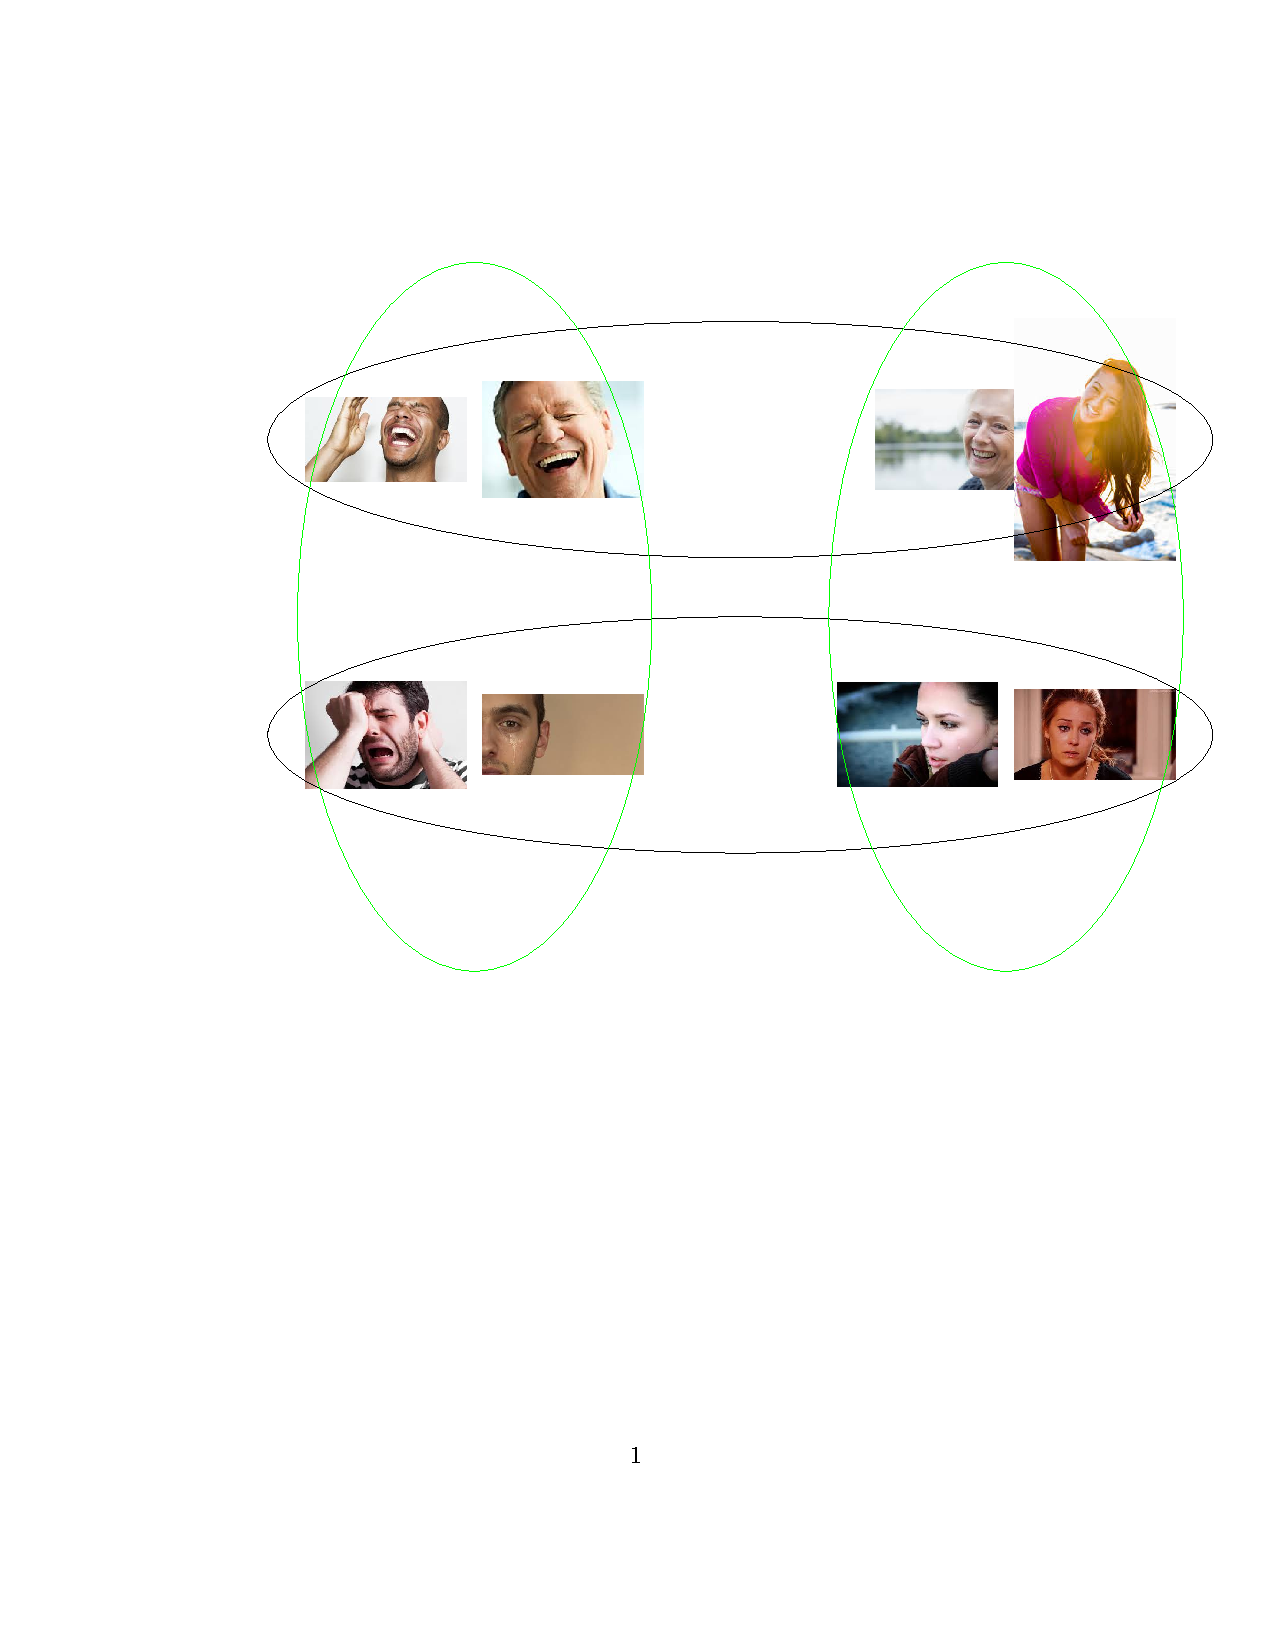
\includegraphics[trim={100 320 30 120},clip,width=0.8\textwidth]{figures/incompatible.pdf}
	\end{center}
\end{frame}

\begin{frame}{The problem of under-specificity}
	Complete information is not available
	\vspace{2cm}

	How to prefer one choice over the other?
\end{frame}

\begin{frame}{Related work}
	Previous approaches to tackle
	\vspace{0.3cm}\begin{itemize}
		\vspace{0.3cm}\item computational complexity 
		\vspace{0.3cm}{\color{lb} \MyCitem under-specificity}
	\end{itemize}
\end{frame}

\begin{frame}{Handling computational complexity}
	Clustering on {\color{green}nice} data is {easy}.\\
	\vspace{1cm}What is nice data?
	\begin{itemize}
		\vspace{0.3cm}\item $\alpha$-center proximity
		\vspace{0.3cm}\item Weak deletion stability
		\vspace{0.3cm}\item $\epsilon$-separatedness
		\vspace{0.3cm}\item $\lambda$-center separation		
	\end{itemize}
\end{frame}

\begin{frame}{Center proximity}
	\begin{center}
	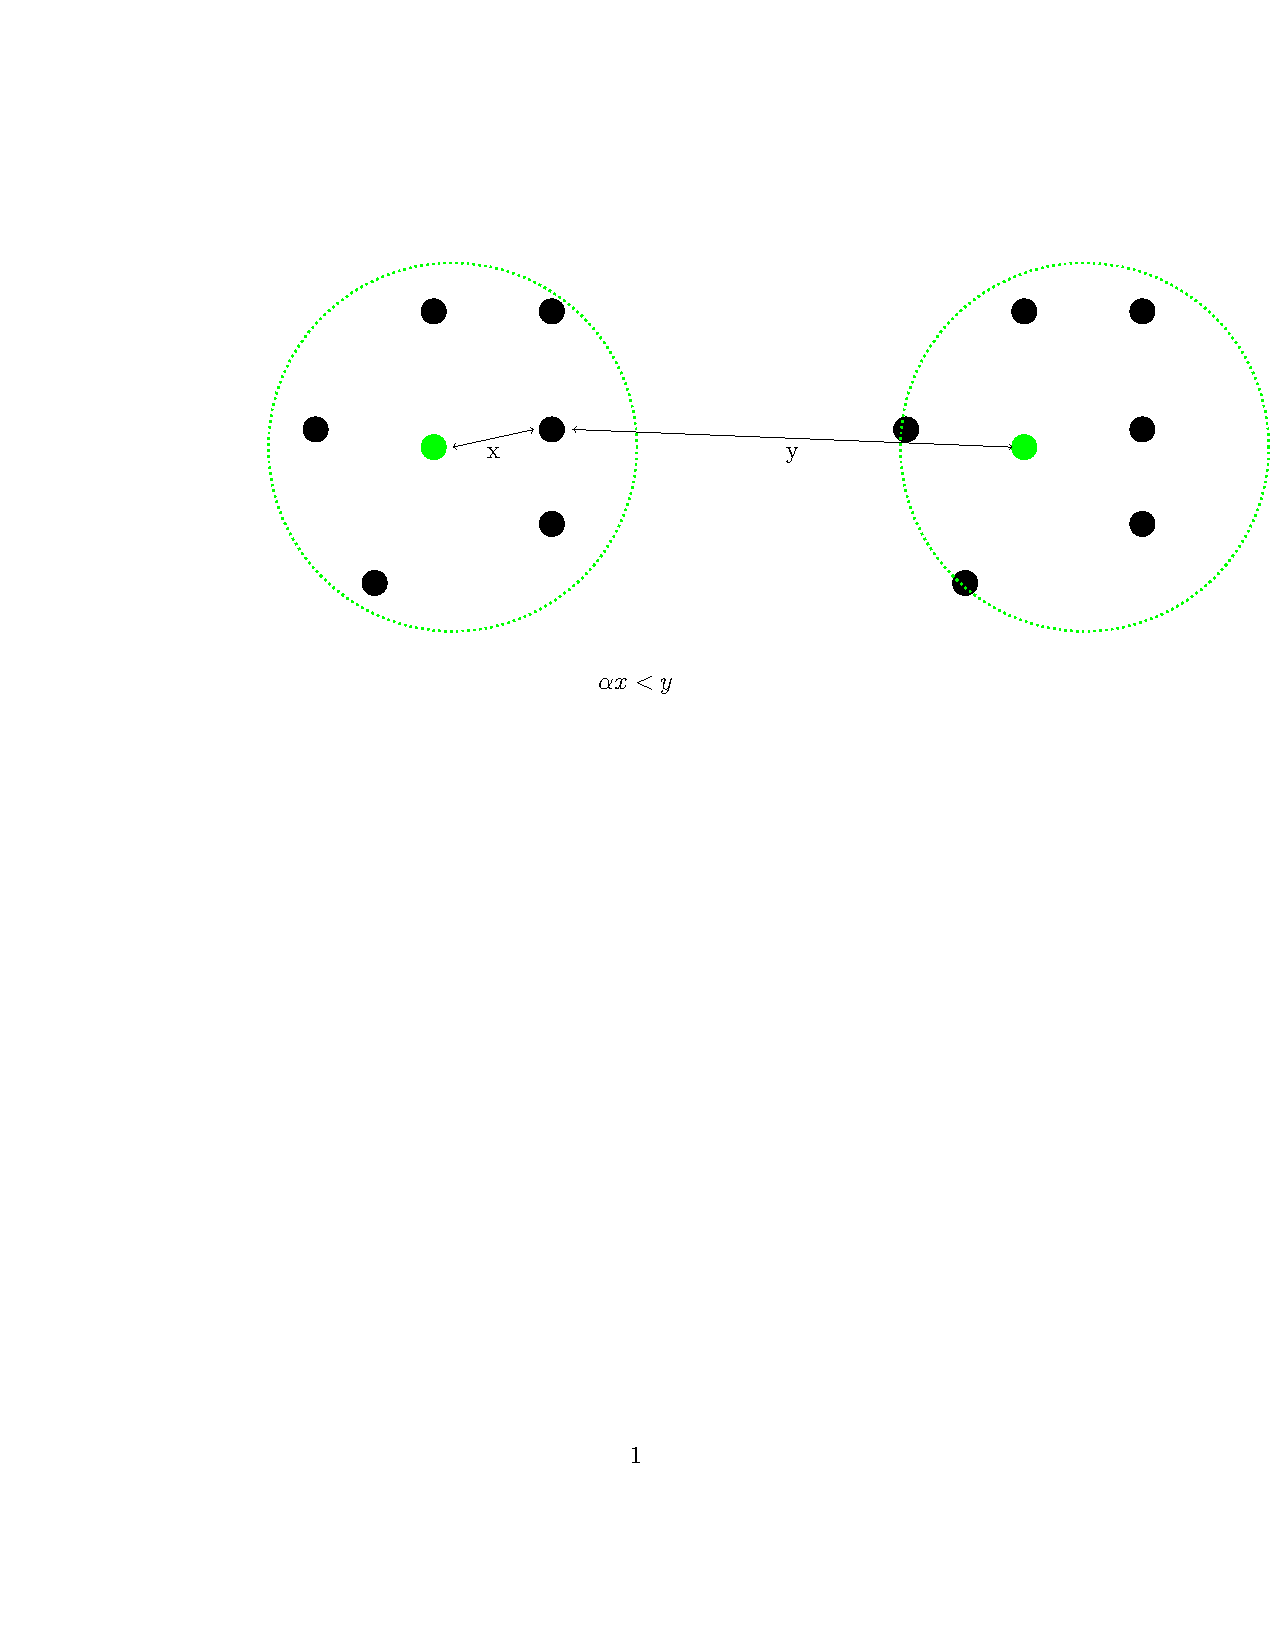
\includegraphics[trim={120 430 0 120},clip,width=0.7\textwidth]{figures/alphacp.pdf}
	\end{center}
	
	\begin{itemize}
		\item Efficiently solvable for $\alpha > 2.4$
		\item NP-Hard for $\alpha < 2$.
		\vspace{0.5cm}\item $\alpha = 2$ already \alert{unrealistic}.
	\end{itemize}
\end{frame}

\begin{frame}{Other clusterability notions}
	$\epsilon$-separatedness\\
	\begin{center}Cost(Opt(k)) $< \epsilon^2$Cost$(Opt(k-1))$\end{center}
	\begin{itemize}
		\item Can {\color{blue} explain success} of Lloyd's algorithm 
		\item \alert{Very strict} assumptions on data $(\alpha > 200)$
	\end{itemize}
	
	\vspace{0.5cm} WDS is similar to $\epsilon$-separatedness\\

	\vspace{0.5cm}$\lambda$-center separation
	\begin{itemize}
	\item Can somewhat {\color{blue} explain success} of $k$-means but \alert{very restrictive}.	 
	\end{itemize}
\end{frame}

\begin{frame}{In conclusion}
Various notions of clusterability.\\
\vspace{1cm}None are both {\color{blue}realistic} and {\color{blue}efficient}.\\
\vspace{1cm}Some can explain popular heuristics. But for unrealistic data. 
\end{frame}

\begin{frame}{Related work}
	Previous approaches to tackle
	\vspace{0.3cm}\begin{itemize}
		\vspace{0.3cm}{\color{lb} \MyCitem computational complexity }
		\vspace{0.3cm}\item under-specificity
	\end{itemize}
\end{frame}

\begin{frame}{Handling under-specificity}
  Get \alert{advice} from an expert
  \begin{itemize}
        \vspace{0.3cm}\item User provides \textbf{must/cannot} link constraints.    
        \vspace{0.3cm}\item Small sample clustering
        \vspace{0.3cm}\item \textbf{Merge-split} queries.
  \end{itemize}
  
  \vspace{1.5cm}None of them {\color{blue}realistic} and provably {\color{blue}efficient}.
\end{frame}

\begin{frame}{Current work}
	Our approach to tackle
	\vspace{0.3cm}\begin{itemize}
		\vspace{0.3cm}\item computational complexity
		\vspace{0.3cm}{\color{lb} \MyCitem under-specificity }
	\end{itemize}
\end{frame}

\begin{frame}{Realistic clusterability notion}
	Allows for a subset of \alert{background noise}\\
	
	\vspace{1.2cm}Data $\mc X$ consists of 
	\begin{itemize}
	\vspace{0.5cm}
	\item "well clustered" subset $\mc S$ and 
	\vspace{0.5cm}
	\item "unstructured" complement $\mc Y= \mc X \setminus \mc S$,
	\end{itemize}
\end{frame}

\begin{frame}{Our definition: \alert {Sparse Noise}}
	\vspace{0.2cm}Any ball of small radius contains few points from $\mc Y$.
    \begin{figure}
	  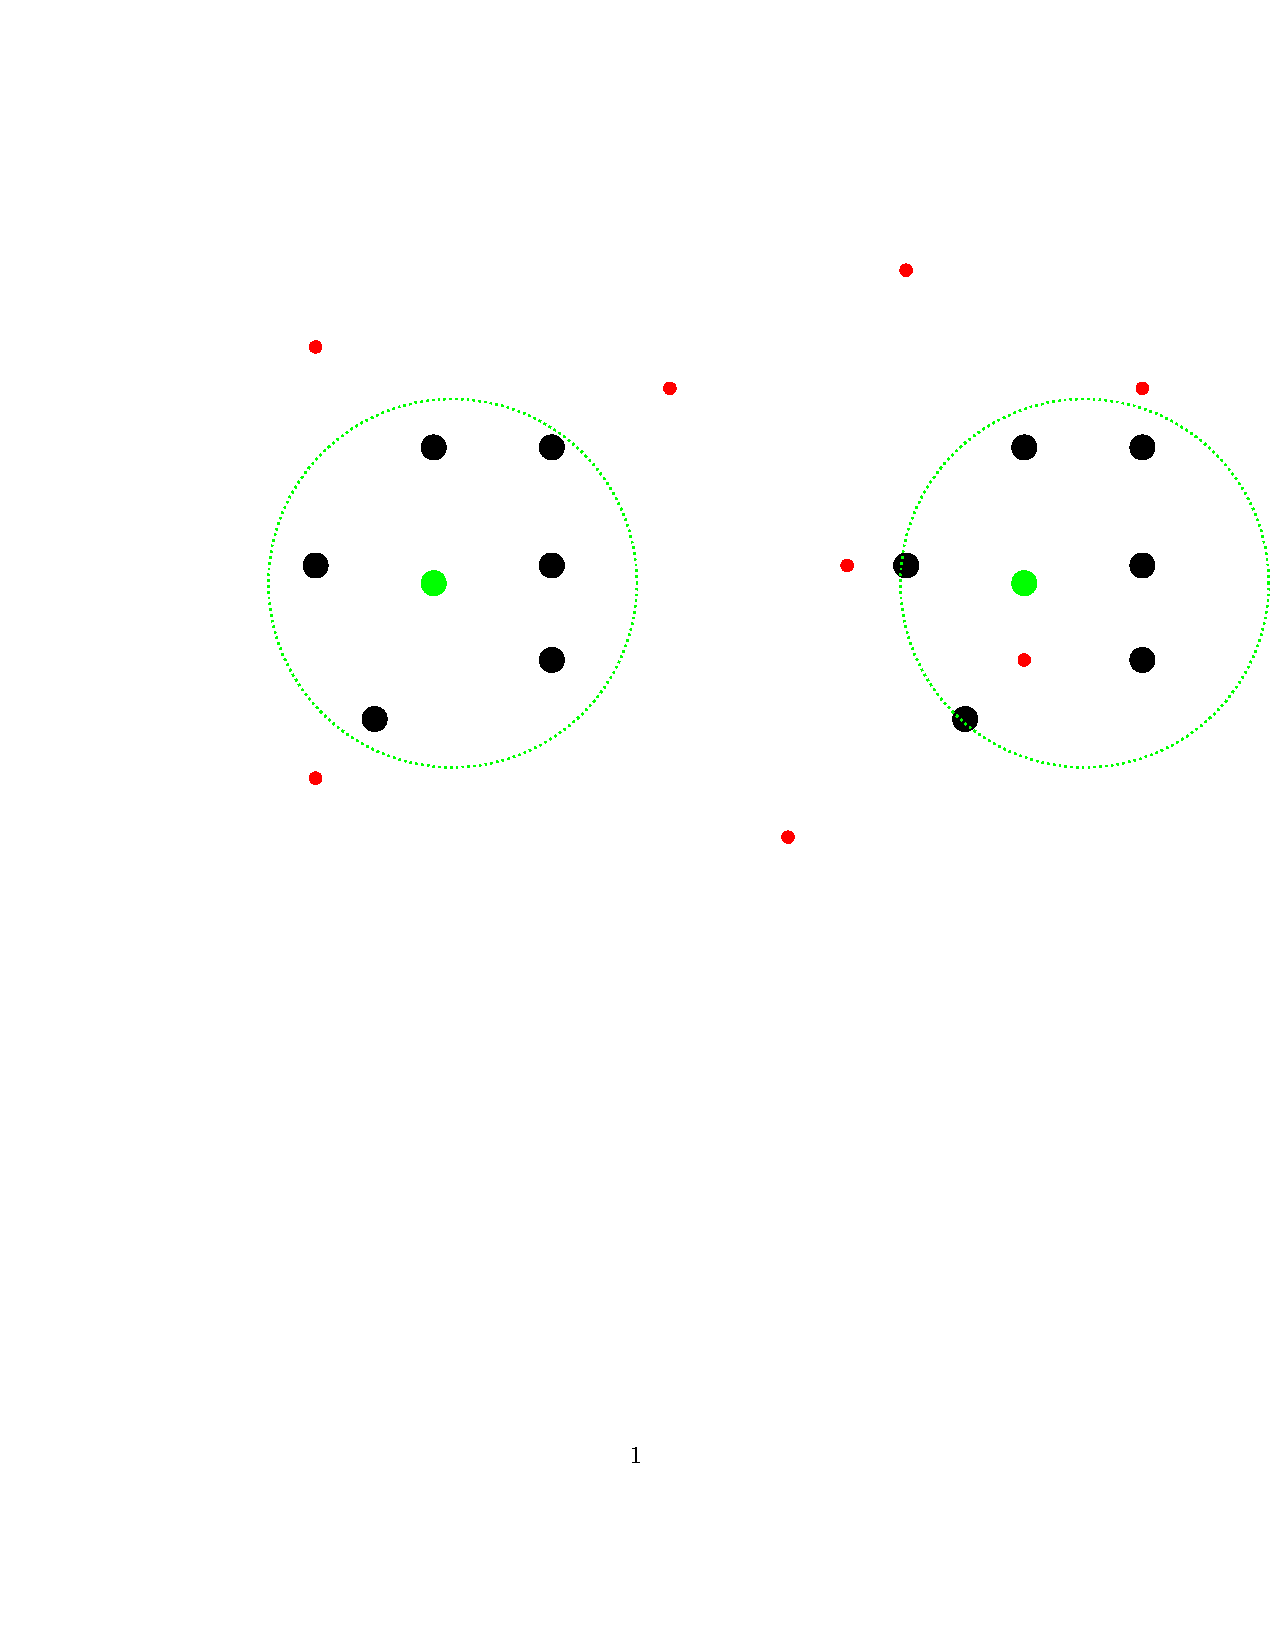
\includegraphics[trim = 100 0 0 100, clip, width=0.8\linewidth]{figures/alphacpnoise.pdf}
   \end{figure}
\end{frame}

\begin{frame}{Current work}
	Our approach to tackle
	\vspace{0.3cm}\begin{itemize}
		\vspace{0.3cm}{\color{lb} \MyCitem  computational complexity}
		\vspace{0.3cm}\item under-specificity
	\end{itemize}
\end{frame}

\begin{frame}{Same-cluster query}
    Do $x_1$ and $x_2$ belong to the same cluster?\\
    \begin{center}
	
\includegraphics[width=0.25\linewidth]{figures/ml1.jpeg}
	\hspace{0.3in}
\includegraphics[width=0.15\linewidth]{figures/eqQues.jpg}\hspace{0.3in}
	
\includegraphics[width=0.15\linewidth]{figures/wl2.jpeg}
    \end{center}
    
	\vspace{1.4cm} Another approach could be to allow {\color{blue}multiple solutions}
\end{frame}

\begin{frame}{Methods}
	We use following methods to address the challenges in clustering.
	\begin{itemize}
		\vspace{0.9cm}\item $\underbrace{\text{Sparse noise}}_{\substack{\text{tackles computational} \\ \text{complexity}}}$ + $\underbrace{\text{multiple solutions}}_{\text{tackles under-specificity}}$
		\vspace{0.9cm}{\color{lb} \MyCitem $\underbrace{\text{Same-cluster query}}_{\text{tackles under-specificity}}$ + $\underbrace{\text{realistic clusterability condition}}_{\substack{\text{tackles computational} \\ \text{complexity}}}$ }
	\end{itemize}
\end{frame}

\begin{frame}{A high level problem description}

	Design algorithms that get a data set with a metric $(\mc X, d)$ so that
	\vspace{1cm}
	\begin{itemize}
		\item Assuming the data consists of 
		\begin{itemize}
		\vspace{0.5cm}
		\item subset $\mc S$ satisfying $\alpha$-center proximity 
		\vspace{0.5cm}
		\item complement $\mc Y= \mc X \setminus \mc S$ is sparse,
		\end{itemize}

		\vspace{1.5cm}
		\item Outputs a partition $C=(C_1, \ldots C_k)$ that \emph{induces} a good clustering of $\mc S$.
	\end{itemize}
\end{frame}

\begin{frame}{Sparse noise definition}
    \begin{figure}
	  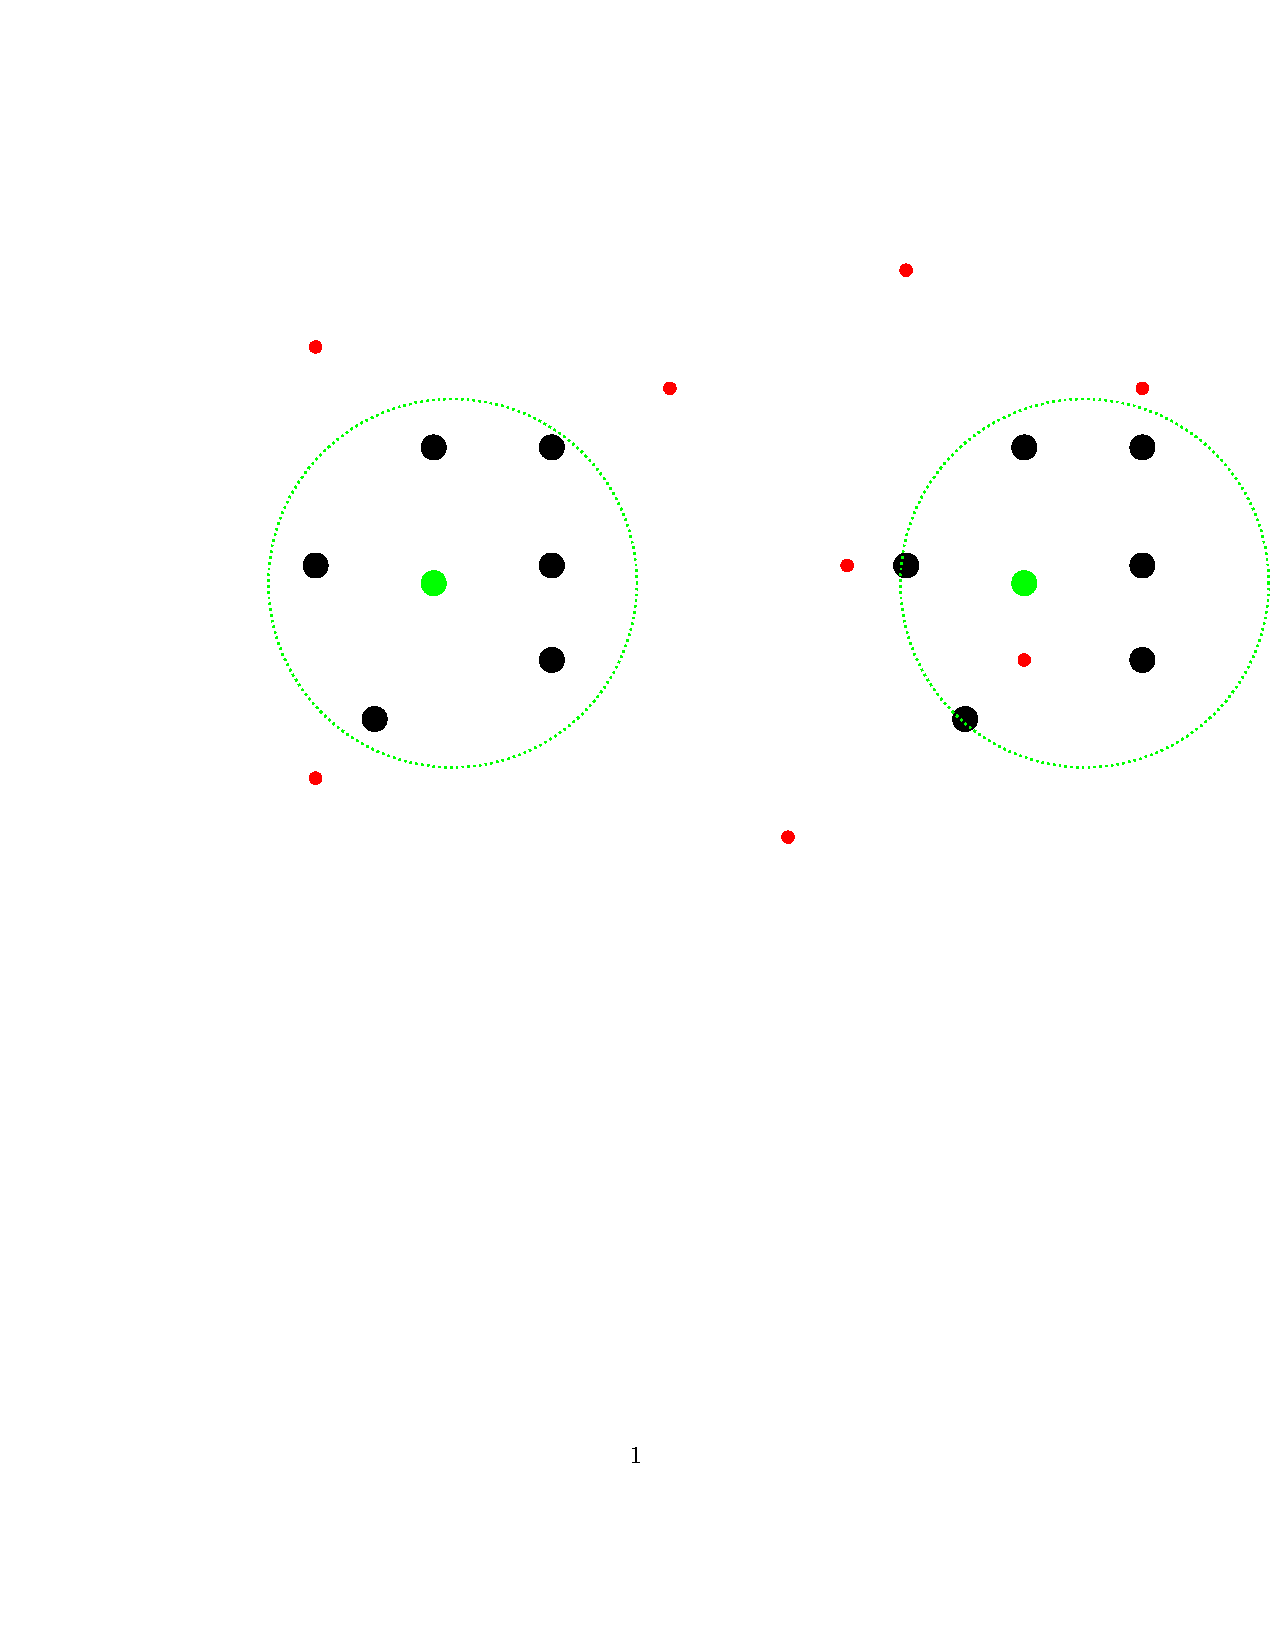
\includegraphics[trim = 100 0 0 100, clip, width=0.8\linewidth]{figures/alphacpnoise.pdf}
   \end{figure}

\end{frame}

\begin{frame}{Our Results}
 \alert{Positive results}
 \begin{itemize}
  	\item $\alpha > 4.6$ and noise is sparse\\ 	
	\textcolor{blue}{We construct  in poly time a clustering tree that induces the original nice clustering}.  	
	\begin{figure}
	  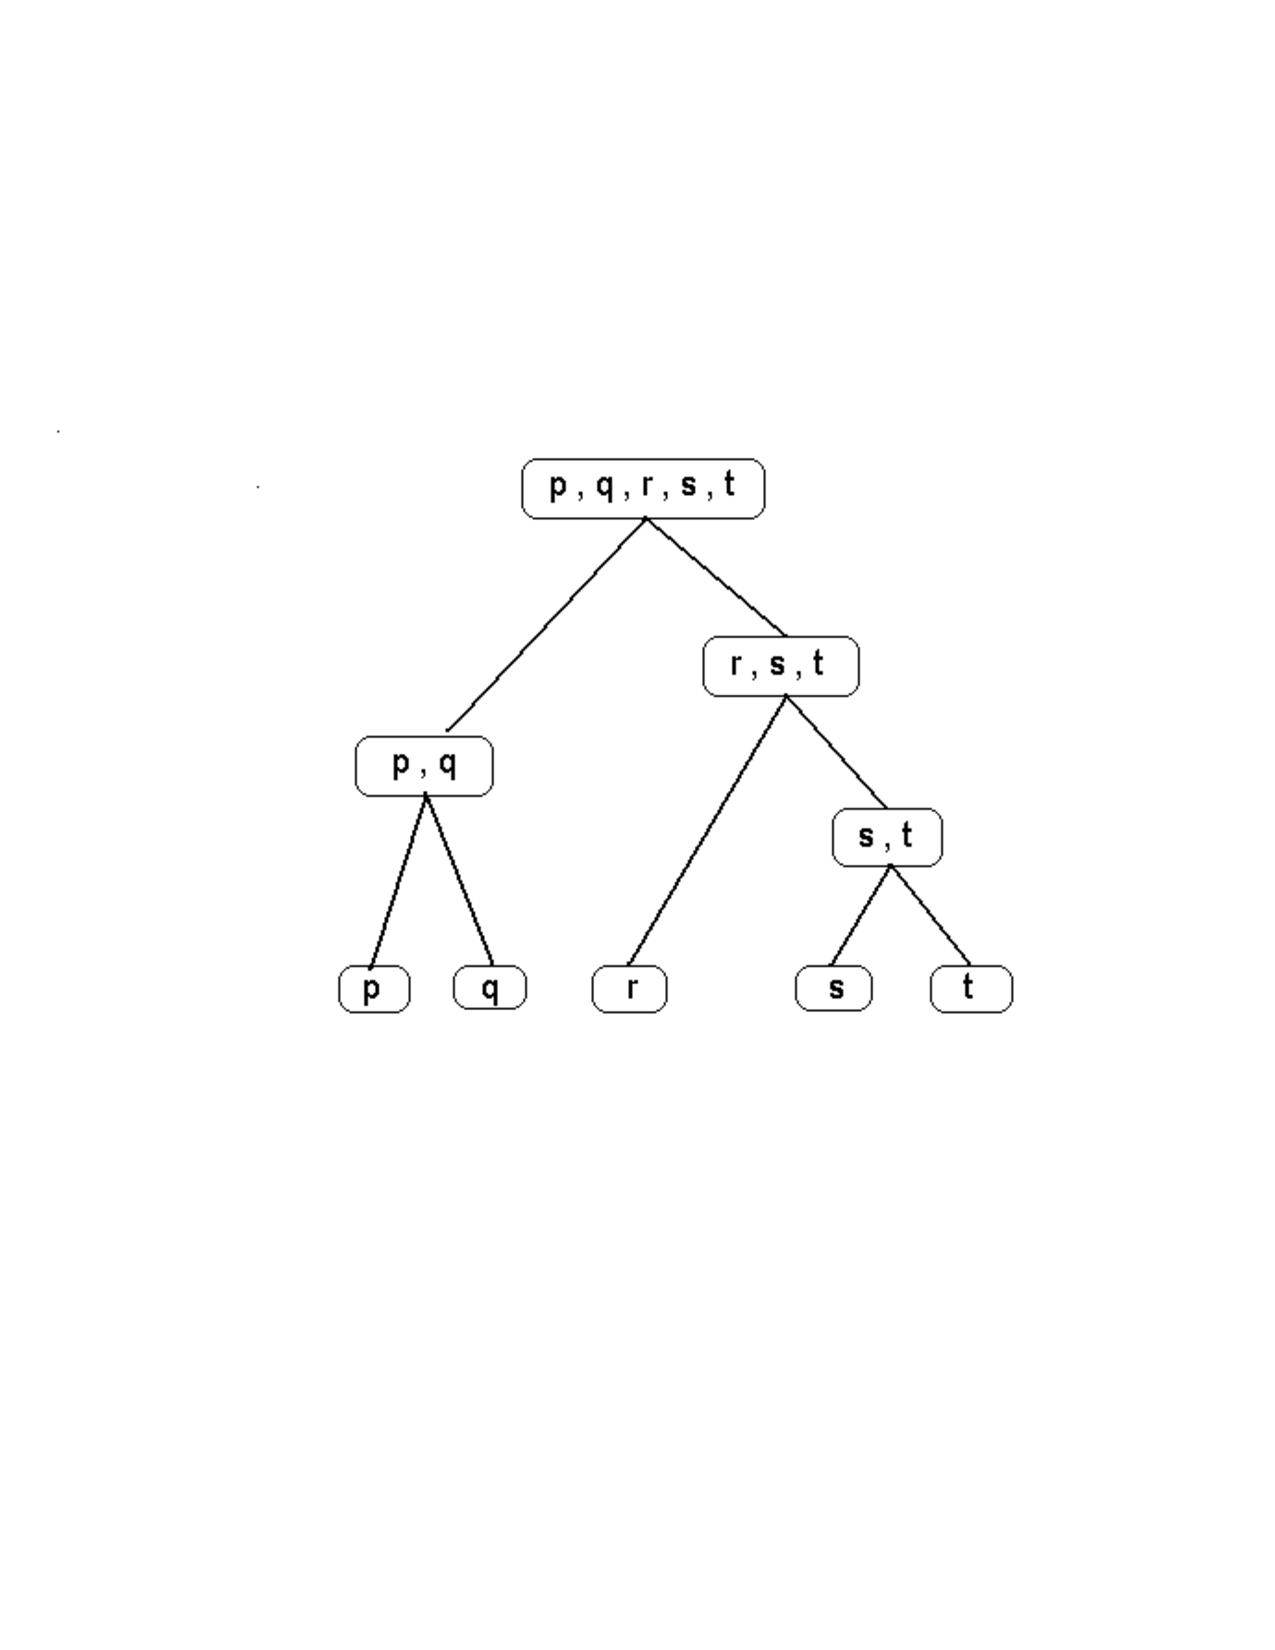
\includegraphics[trim = 50 150 50 200, clip, width=0.8\linewidth]{figures/hier.pdf}
	\end{figure}	  	
  \end{itemize}  
\end{frame}

\begin{frame}{Our Results}
	\alert{Negative results}
  	\begin{itemize}
	  	\vspace{0.5cm}\item $\alpha < 5.8$ and noise is adversarial, or 
		\vspace{0.5cm}\item $\alpha < 4.4$ and noise is sparse
	\end{itemize}
	 \vspace{1.0cm}One cannot guarantee \textcolor{red}{ efficient recovery} of the non-noise clustering. 
\end{frame}

\begin{frame}{Sparse-distance condition}
    We say that the ball $B$ satisfies the sparse distance condition w.r.t clustering $\mc C$ when the following holds.
	\begin{itemize}
	  \item $|B| \ge t$.
	  \item For any $X_i \in \mc C$, if $X_i \cap B \neq \emptyset$, then $X_i \subseteq B$ or $|B \cap X_i| \ge t/2$.
	\end{itemize}

   \begin{figure}
	  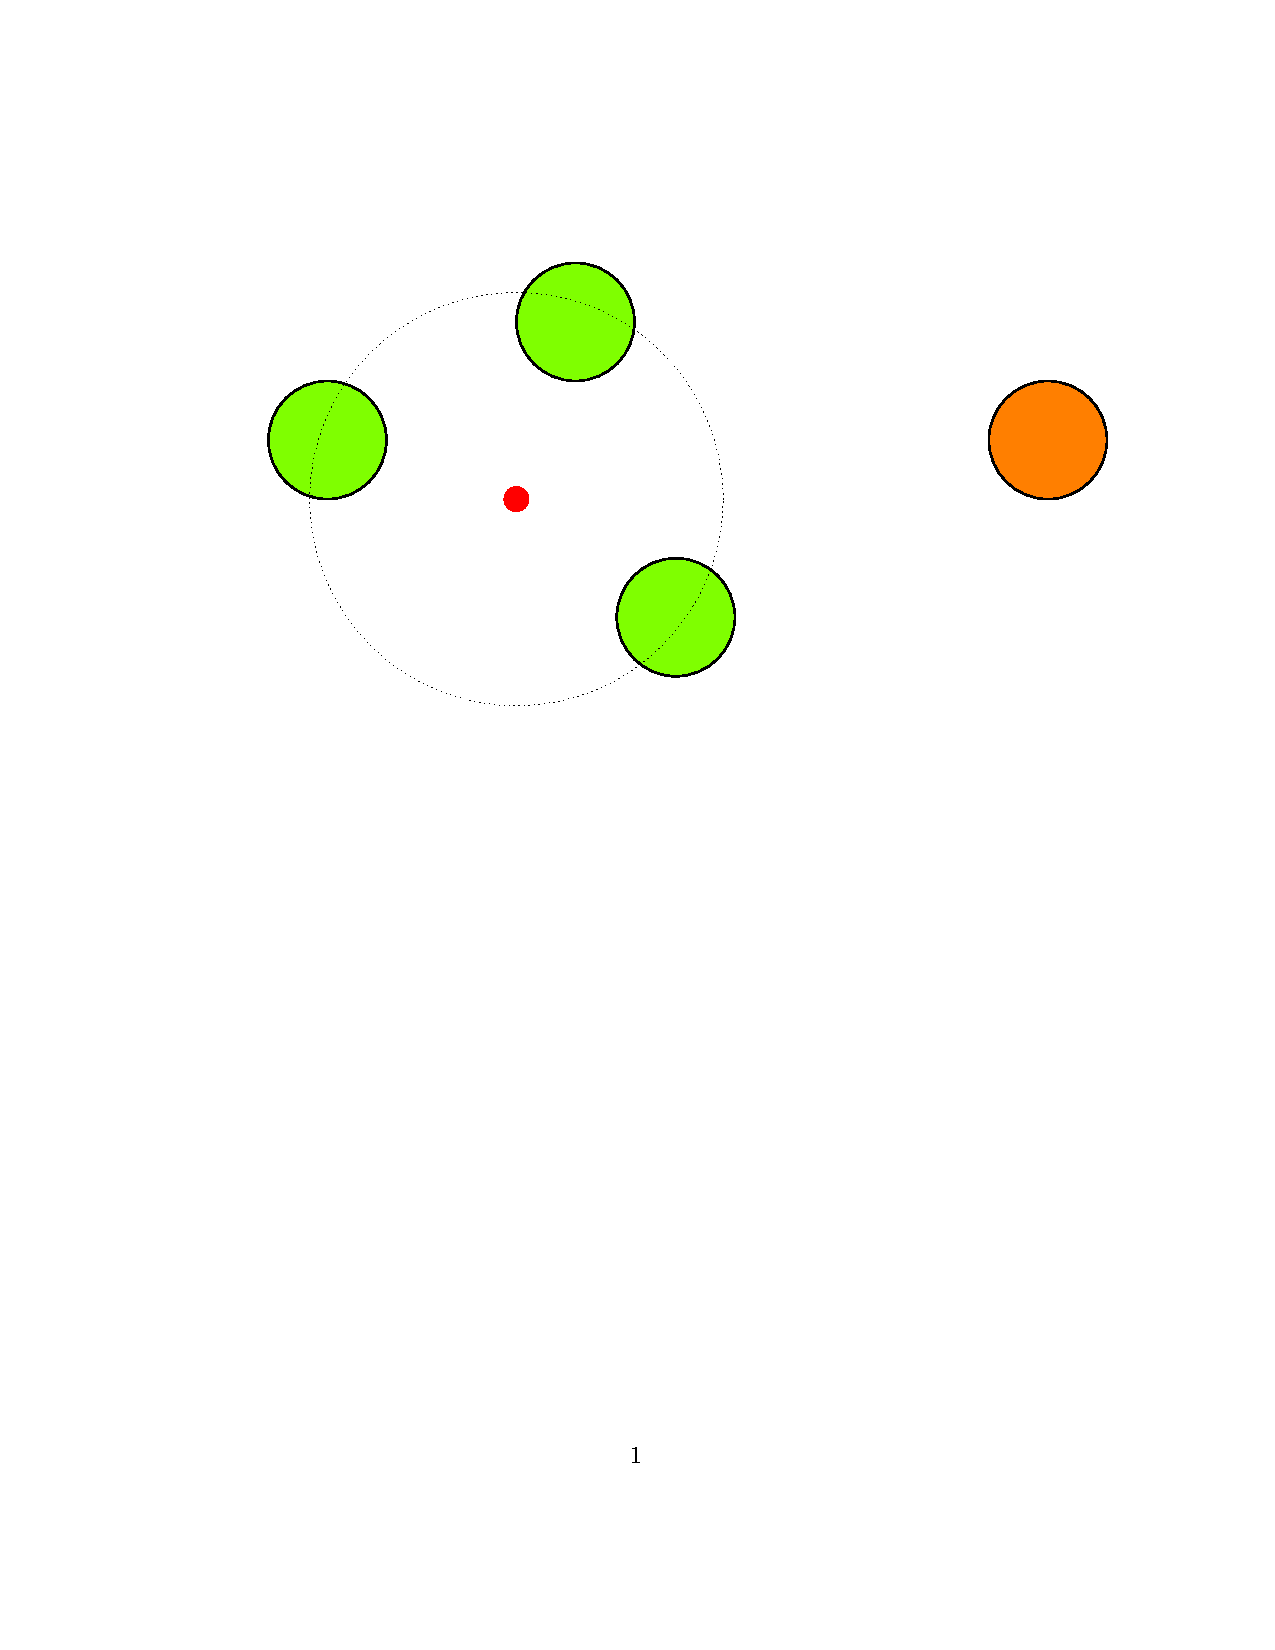
\includegraphics[trim = 100 0 0 100, clip, width=\linewidth]{figures/sparseDistanceSatisfied.pdf}
   \end{figure}
\end{frame}

\begin{frame}{Sparse-distance condition failure}   
   \begin{figure}
	  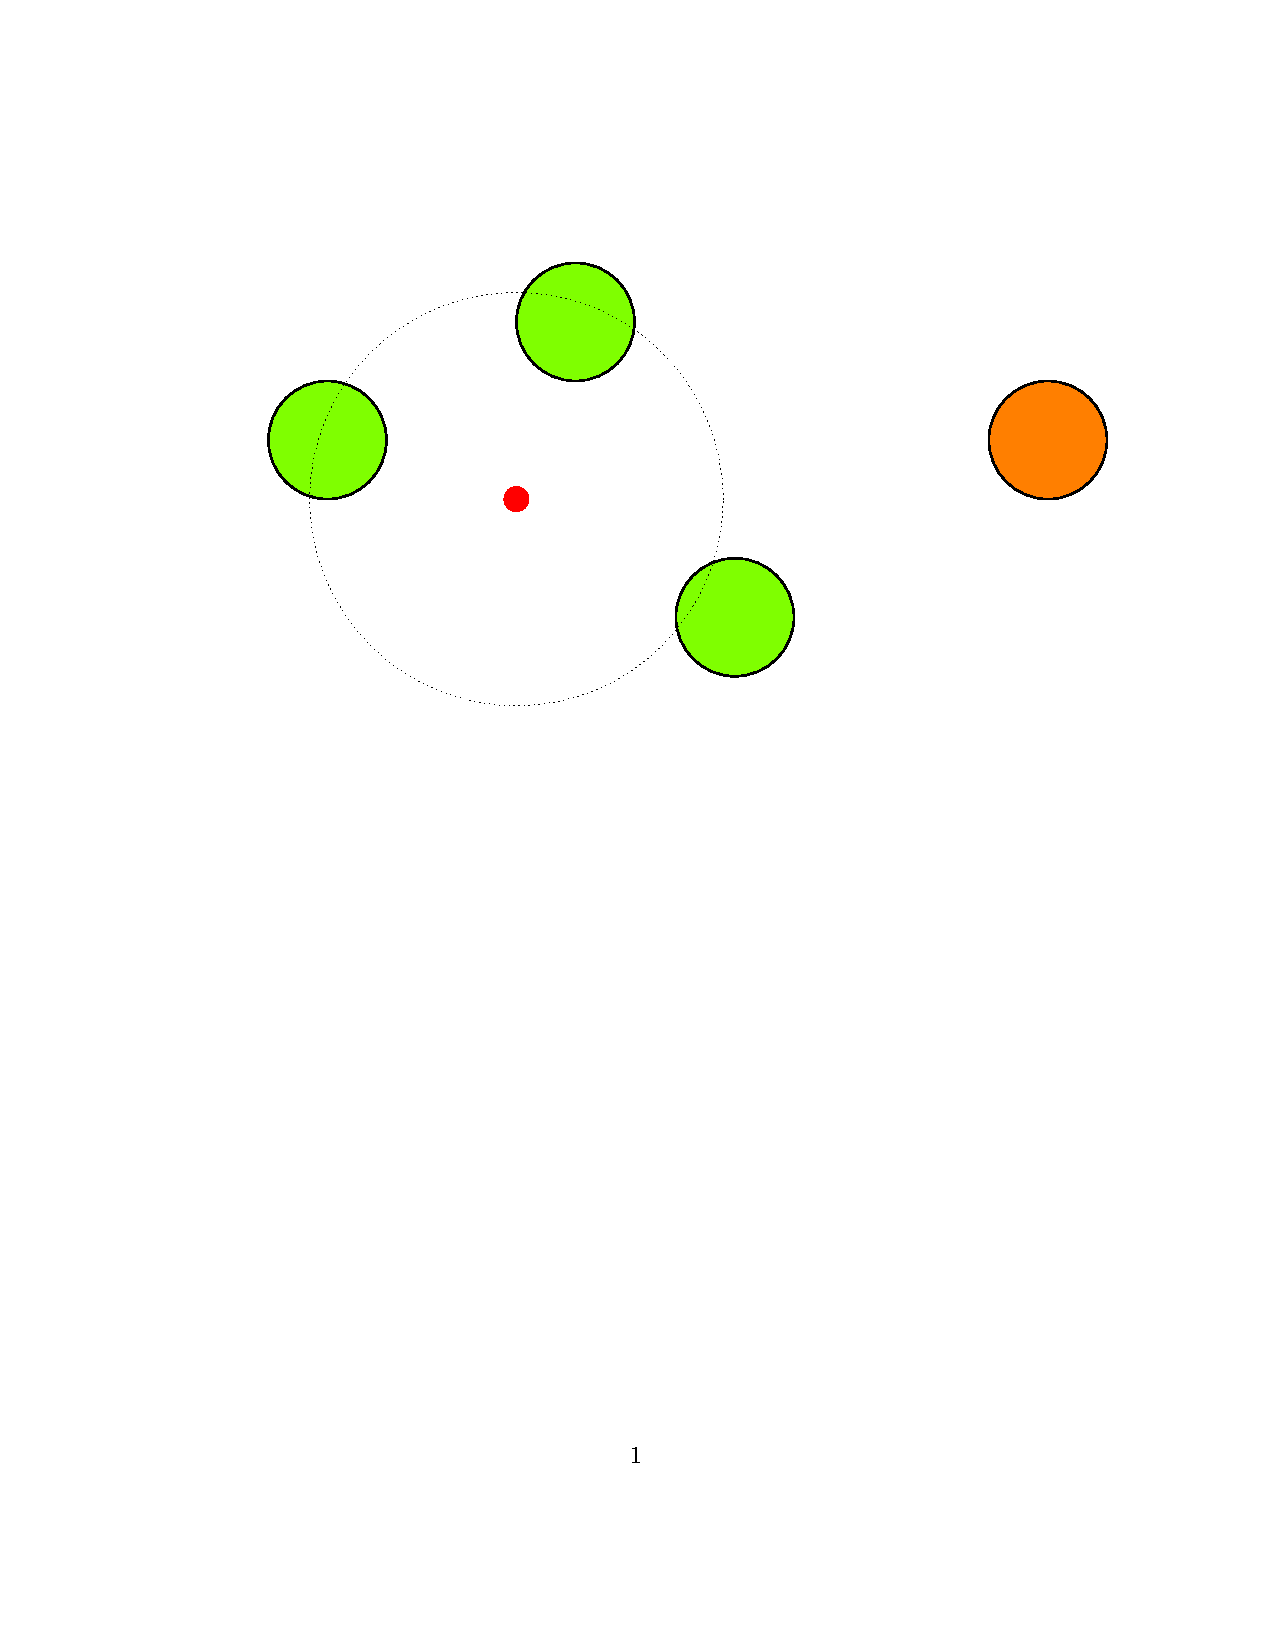
\includegraphics[trim = 100 0 0 100, clip, width=\linewidth]{figures/sparseDistanceNotSatisfied.pdf}
   \end{figure}
\end{frame}


\begin{frame}{Clustering under $(\alpha, \eta)$-center proximity}
	\begin{block}{The algorithm}
	  Input: $(\mc X, d)$ and a parameter $t$.\\
	  Output: A hierarchical clustering tree.\\
	  \vspace{0.1in}Initialize every point in its own cluster.\\
	  Go over all pairs of points $p, q$ in increasing order of distance.\\
	  If $B := B(p, d(p, q))$ satisfies the sparse-distance condition
	  \begin{itemize}
	  	\item Merge all clusters that intersect with $B$ into a single cluster
	  \end{itemize}
    \end{block}
\end{frame}

\begin{frame}{Lower bound}
	If $\alpha < 3 + \sqrt{2}$ and noise is sparse, then there doesn't exist a clustering tree which can capture all nice solutions.
	\begin{figure}[!t]
	  \begin{center}
	    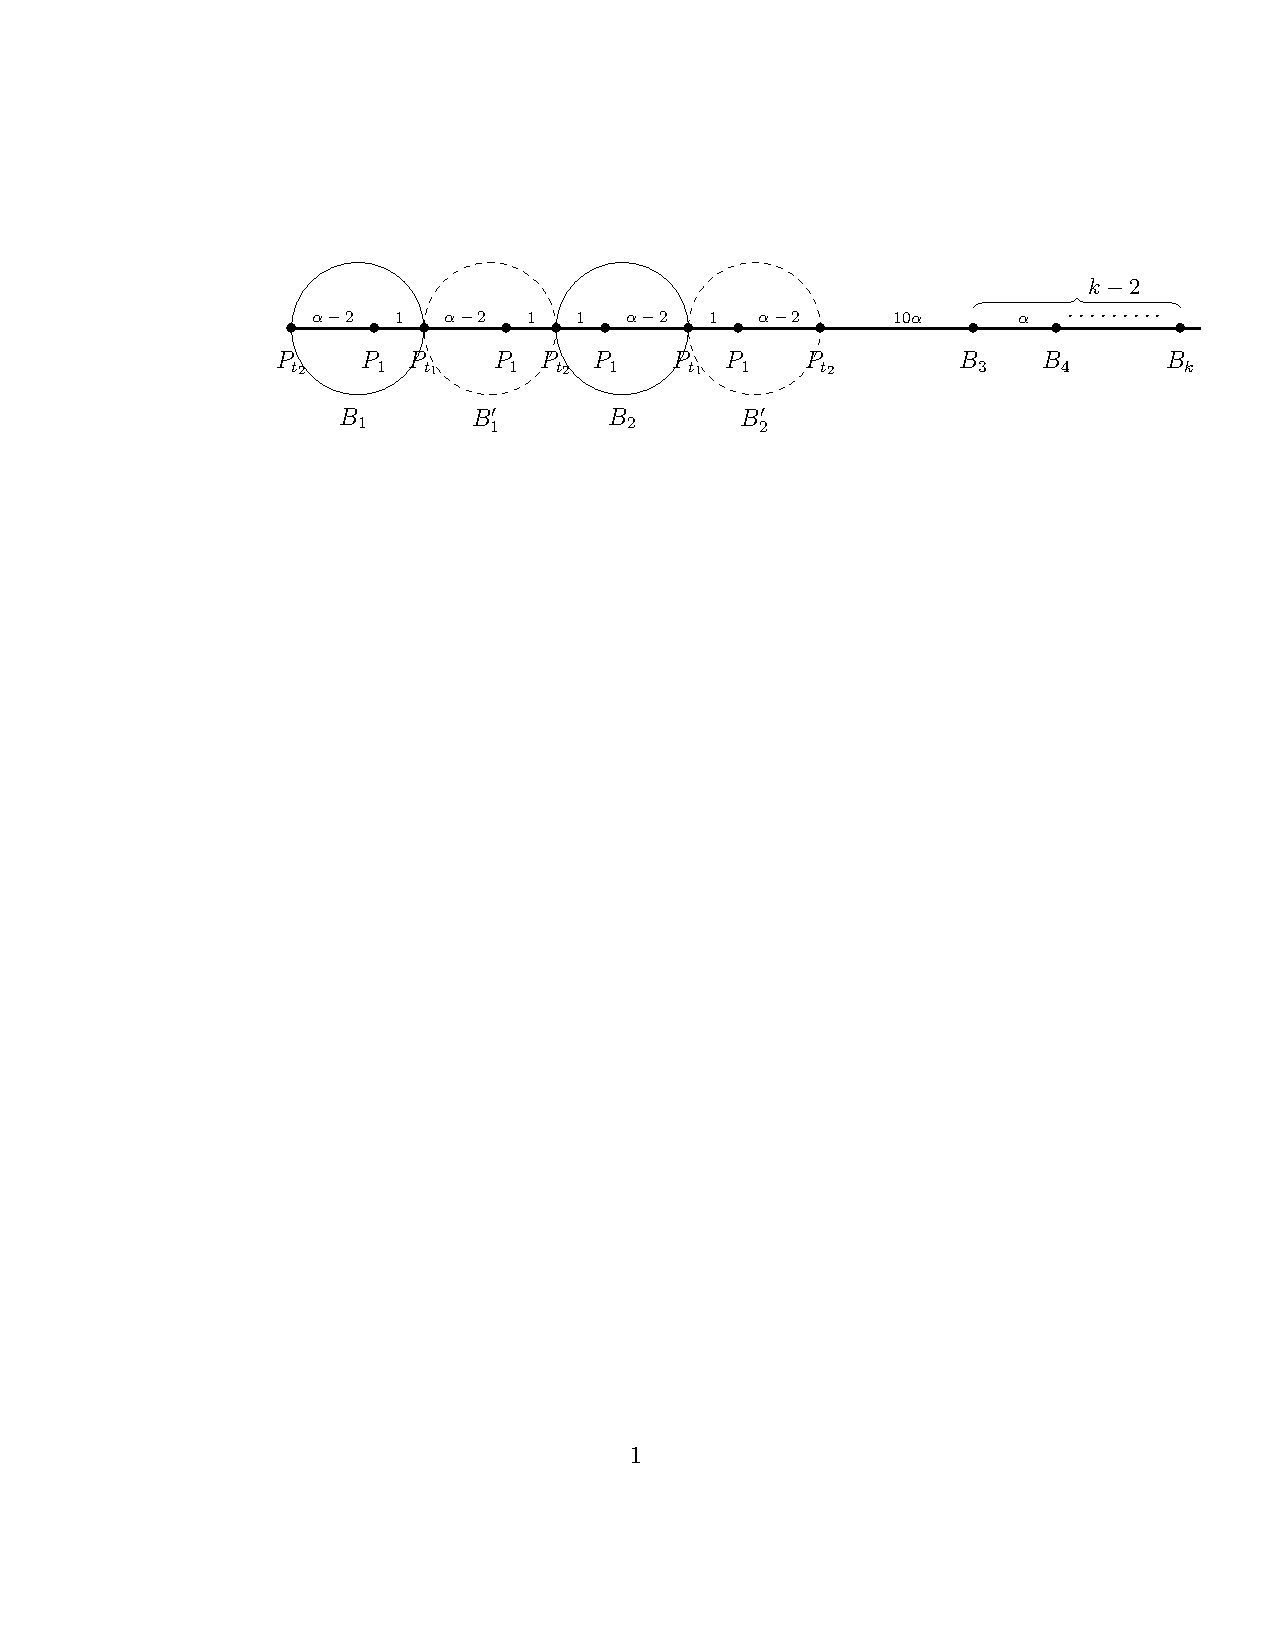
\includegraphics[trim={47mm 205mm 12mm 44mm},clip,width=\textwidth]{figures/lbdFig2.pdf}
	  \end{center}
	\end{figure}
	Same ideas can be extended to a list output. Any list should have size $> 2^{k/2}$
\end{frame}

\begin{frame}{Methods}
	We use following methods to address the challenges in clustering.
	\begin{itemize}
		\vspace{0.9cm}{\color{lb} \MyCitem $\underbrace{\text{Sparse noise}}_{\substack{\text{tackles computational} \\ \text{complexity}}}$ + $\underbrace{\text{multiple solutions}}_{\text{tackles under-specificity}}$}
		\vspace{0.9cm}\item $\underbrace{\text{Same-cluster query}}_{\text{tackles under-specificity}}$ + $\underbrace{\text{realistic clusterability condition}}_{\substack{\text{tackles computational} \\ \text{complexity}}}$ 
	\end{itemize}
\end{frame}


\begin{frame}{A high level problem description}
	Design algorithms that get a data set with a metric $(\mc X, d)$ so that
	\vspace{1cm}
	\begin{itemize}
		\item Assuming that data satisfies $\gamma$-margin
		\vspace{1.0cm}
		\item Output the true partition $C=(C_1, \ldots C_k)$.
		\vspace{1.0cm}
		\item The learner can make same-cluster queries to an oracle.
	\end{itemize}
\end{frame}

\begin{frame}{$\gamma$-margin property}
	\begin{center}        
	    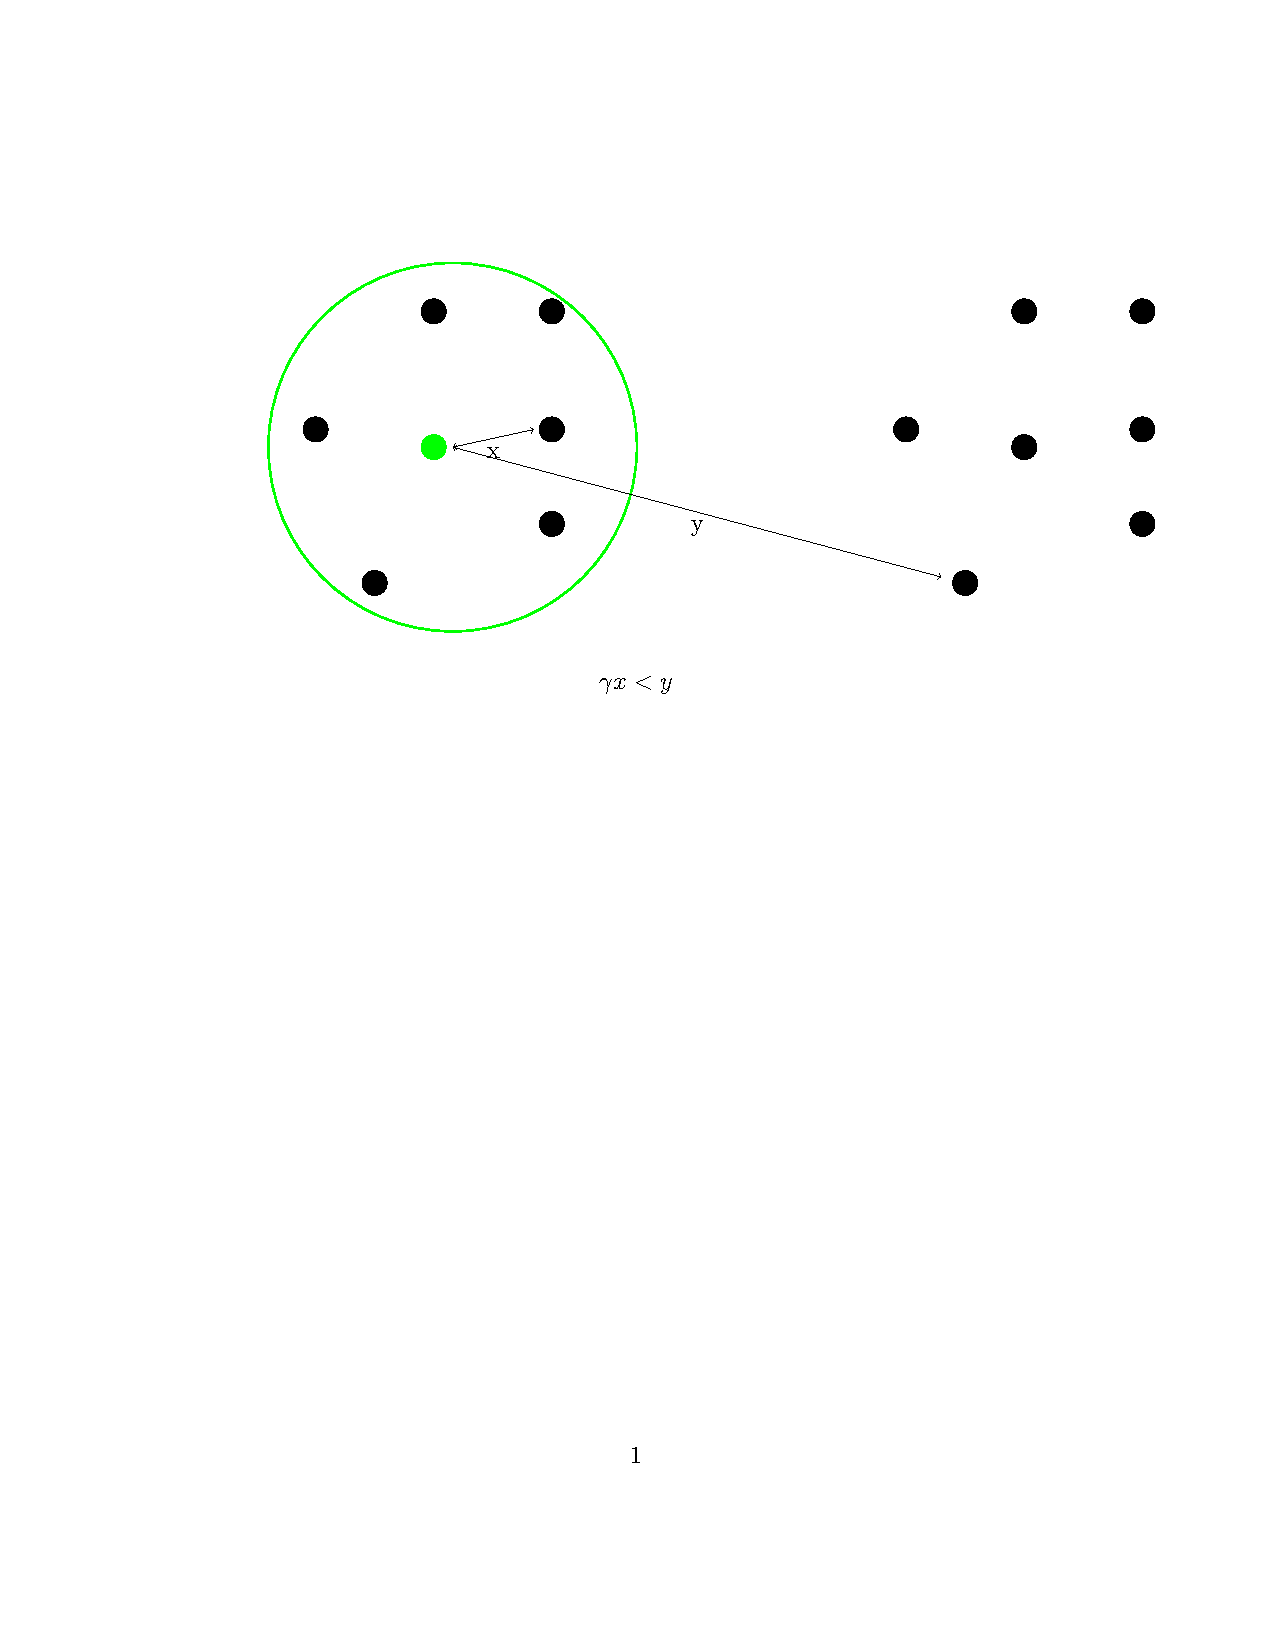
\includegraphics[trim=500 470 500 190,scale=0.5]{figures/gammaMargin.pdf}
    \end{center}    
    
    \begin{block}{}
    $\mc C_{\mc X} = \{C_1, \ldots, C_k\}$ with centers $\{\mu_1, \mu_2, \ldots , \mu_k\}$ satisfies the $\gamma$-margin property if for all $x \in C_i$ and $y \in C_j$,

	$$\gamma d(x, \mu_i) < d(y, \mu_i)$$   
    \end{block}    
\end{frame}

\begin{frame}{$\gamma$-margin without queries}

    \begin{center}        
	    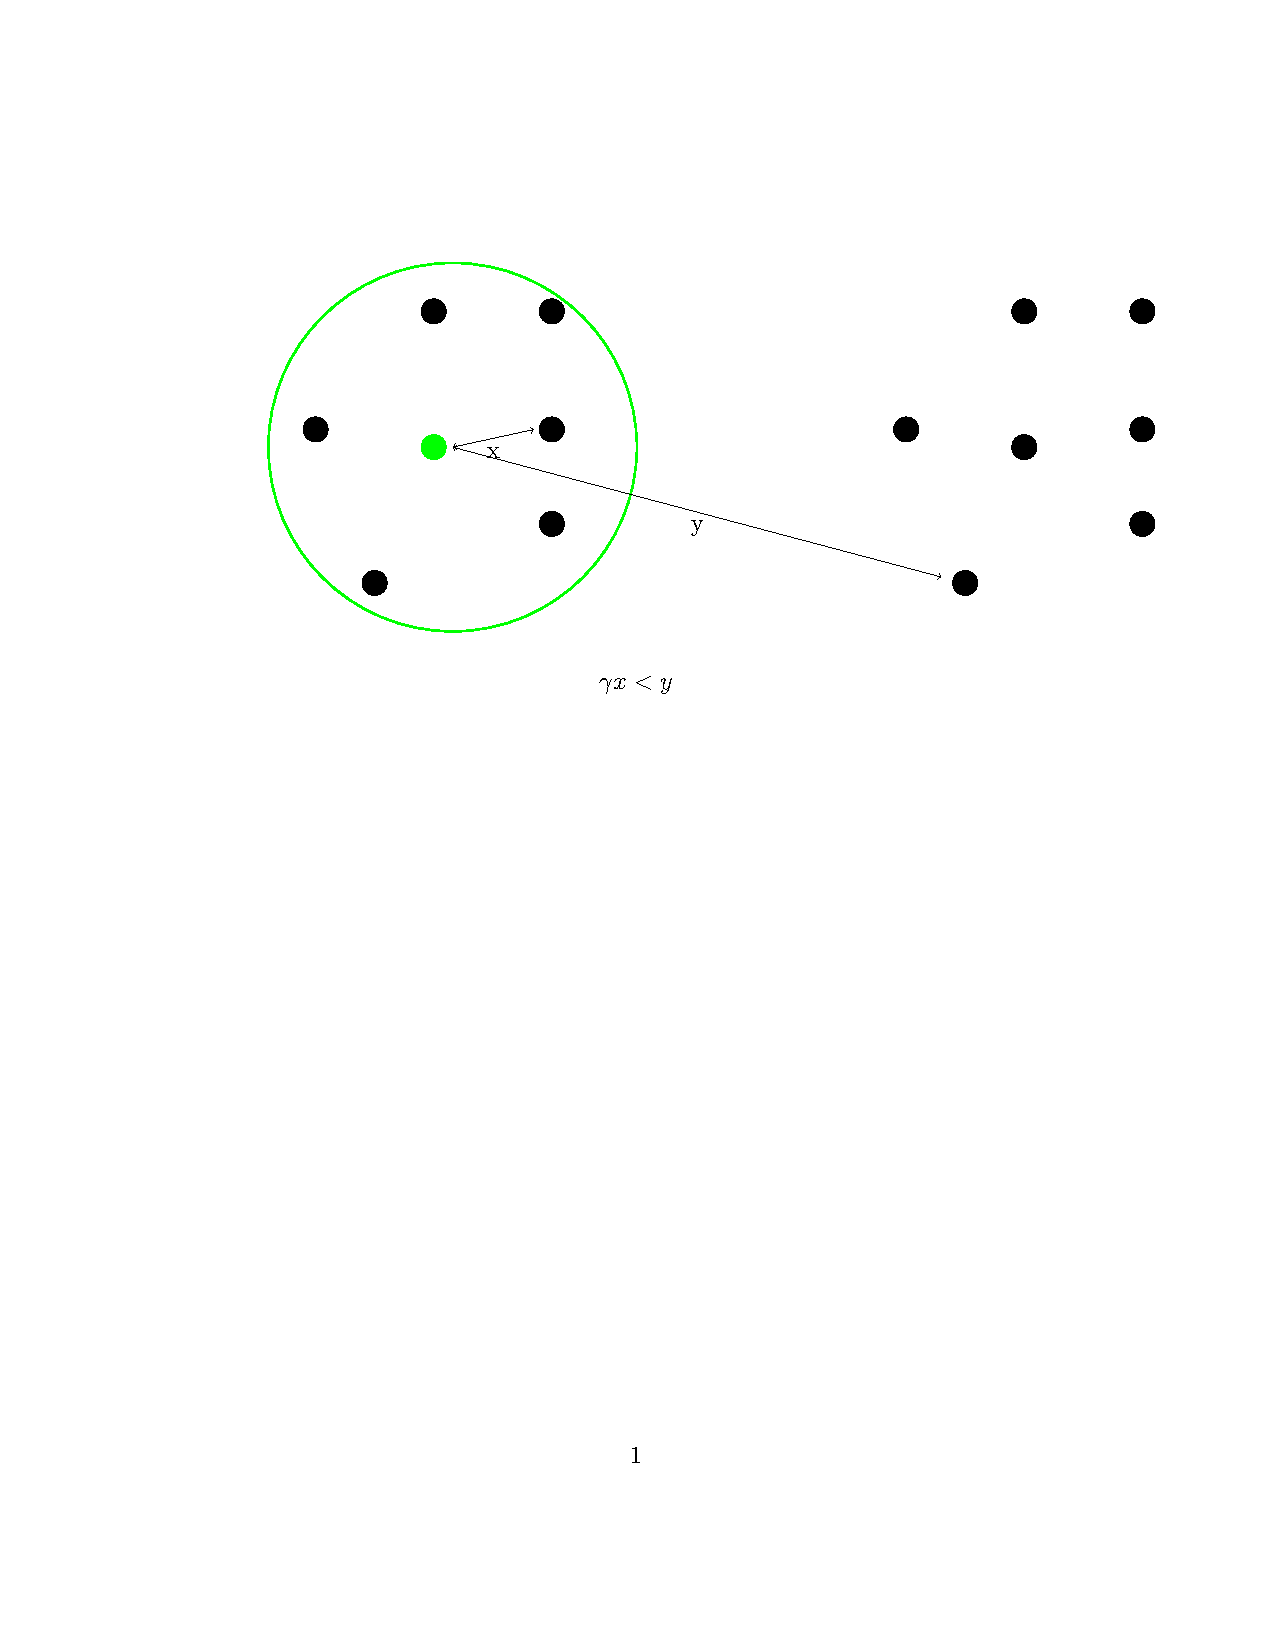
\includegraphics[trim=500 470 500 190,scale=0.5]{figures/gammaMargin.pdf}
    \end{center} 
  
  \vspace{0.5cm}In a ``$k$-median" like setting
  \begin{itemize}
    \vspace{0.3cm}\item {\color{blue} Tractable} for $\gamma > 2$
    \vspace{0.3cm}\item \alert{NP-Hard} for $\gamma < 2$
    \end{itemize}
\end{frame}


\begin{frame}{Our Results}
  \alert{Positive result}
  \vspace{0.5cm}
  \begin{itemize}
    
    \item $\gamma > 1$ \\
    \vspace{0.3cm} \textcolor{blue}{Our algorithm finds the} \textcolor{red}{target} \textcolor{blue}{clustering with high probability}
    
    \begin{itemize}
    	\vspace{0.3cm}
        \item Runs in $O(kn\log n)$
        \vspace{0.3cm}
        \item Asks $O(k^2\log k + k\log n)$ queries
    \end{itemize}
   \end{itemize}
\end{frame}

\begin{frame}{Our results}
	\alert{Negative result} 
	\vspace{0.5cm}
    \begin{itemize}
    \item $\gamma < 1.84$ and no queries.\\
    \vspace{0.3cm} {NP-Hard to find the optimal $k$-means clustering}
    \vspace{0.5cm}
    \item Sub-logarithmic queries don't help.
  \end{itemize}
\end{frame}

\begin{frame}{Key Takeaways}
\begin{itemize}
	\item \textcolor{blue}{Interactive clustering} can tackle \alert{under-specificity} \\
	\vspace{1.0cm}
	\item A few \textcolor{blue}{queries} can make an \textcolor{red}{NP-hard} problem tractable
\end{itemize}
\end{frame}

\begin{frame}{Clustering with queries}
  \begin{block}{The algorithm}
	\vspace{0.2cm}Input: $(\mc X, d)$, $k$ and parameters $\gamma$ and $\delta$.\\
    \vspace{0.2cm}Output: A clustering of $\mc X$.\\
	\vspace{0.3cm}
	\begin{itemize}
	  \item Query uniformly till we have ``enough'' points from one cluster
      \vspace{0.2cm}
	  \item Estimate its center
      \vspace{0.2cm}
	  \item Binary search to find the ``radius"
      \vspace{0.2cm}
	  \item Remove the cluster and repeat
    \end{itemize}  
  \end{block}
\end{frame}

\begin{frame}{The algorithm}   
   \begin{figure}
	  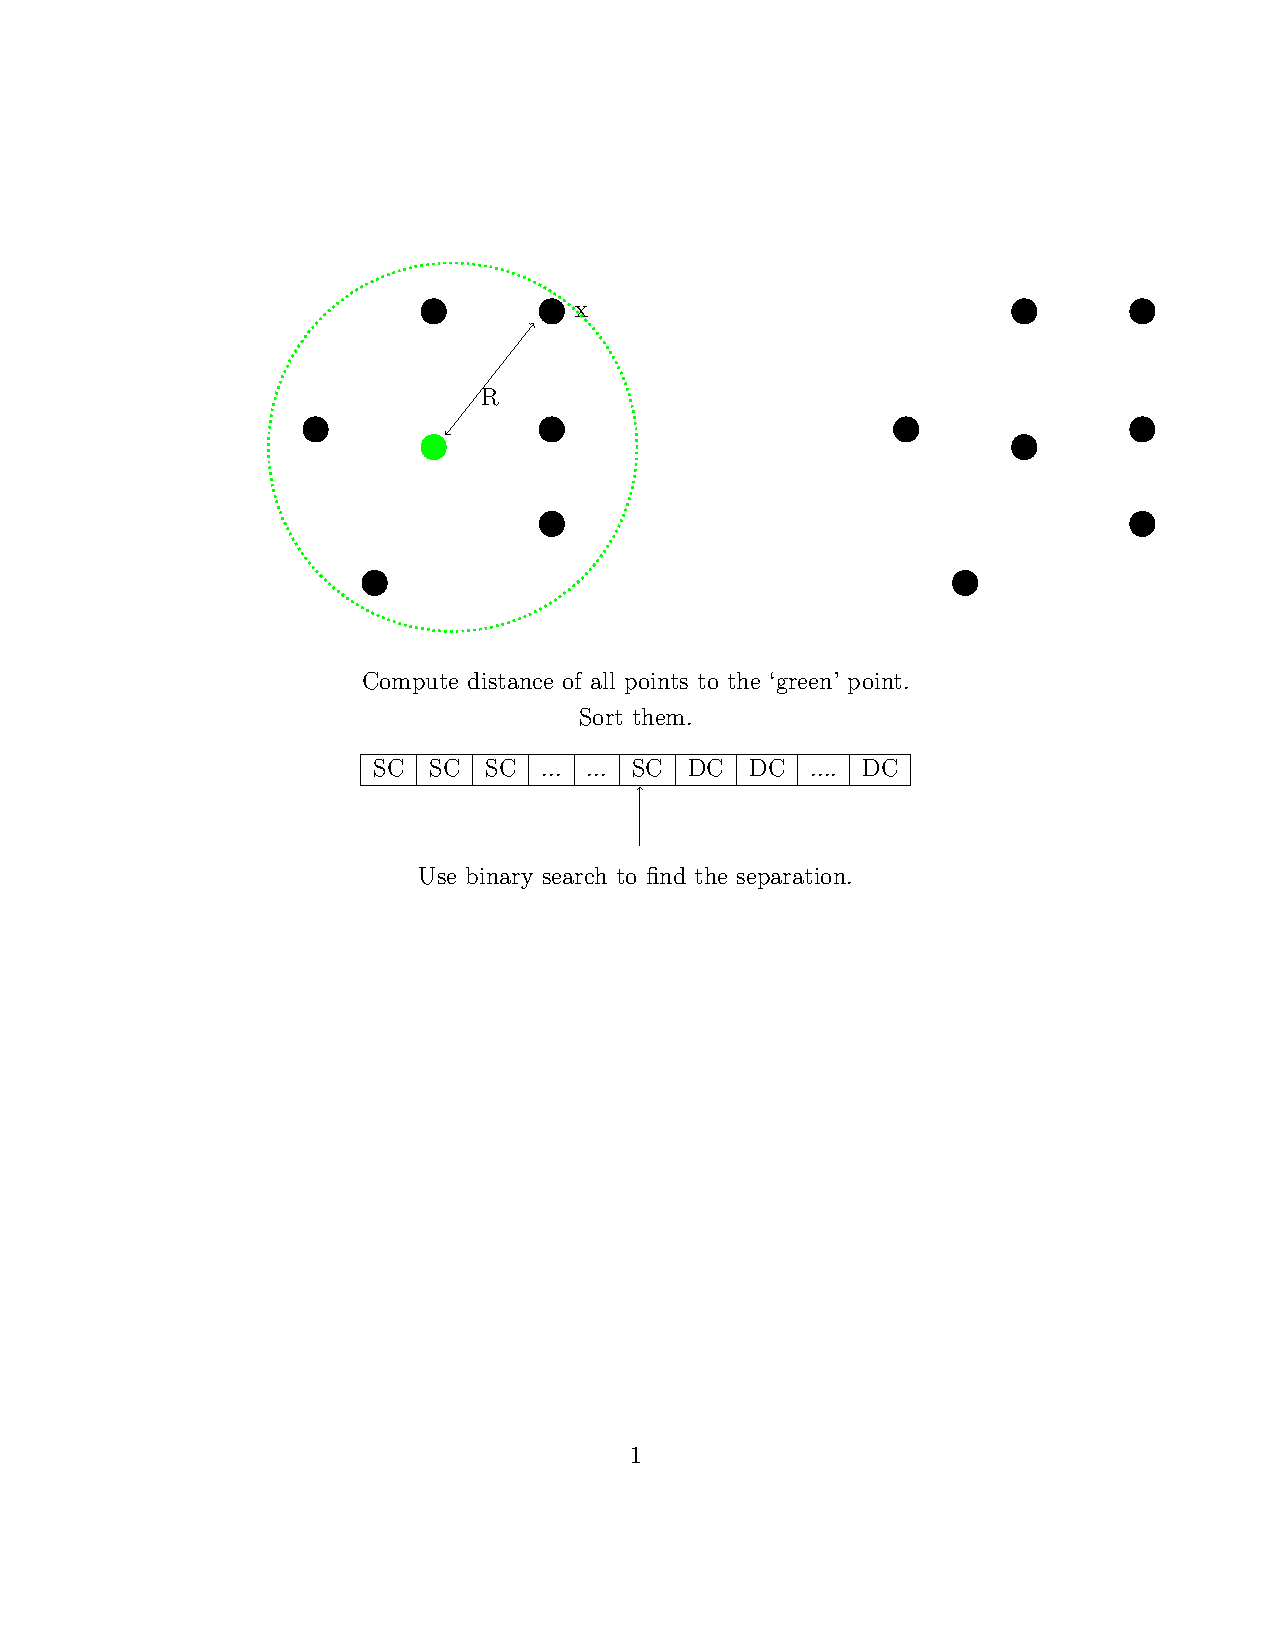
\includegraphics[trim = 100 0 0 120, clip, width=\linewidth]{figures/gammaAlgo.pdf}
   \end{figure}
\end{frame}

\begin{frame}{Lower Bound}
	Euclidean $k$-means is NP-hard even when the optimal solution satisfies the $\gamma$-margin property for $\gamma < 1.84$
	\vspace{0.3cm} 
	\begin{itemize}
		\item Reduction from Exact Cover by 3-Sets ($X3C$).
    	\vspace{0.3cm}\item Hardness for $k = \theta(n^{\epsilon})$
	\end{itemize}
	\pause
	\vspace{0.7cm}Small number of queries
	\vspace{0.3cm}
	\begin{itemize}	
		\item NP-hard with $O(\log n)$ queries
		\vspace{0.3cm}\item Simulation trick
	\end{itemize}	    
\end{frame}

\begin{frame}{Future work}
	Various avenues for future work.
	\begin{itemize}
		\vspace{0.9cm}\item Computational complexity 
		\vspace{0.9cm}{\color{lb} \MyCitem Under-specificity}
	\end{itemize}
\end{frame}

\begin{frame}{Dealing with computational complexity}
	Clusterability notion should be
	\begin{itemize}
		\vspace{0.3cm}\item Realizable
		\vspace{0.3cm}\item Efficient
		\vspace{0.3cm}\item Verifiable
		\vspace{0.3cm}\item Explanation of popular methods
	\end{itemize}
\end{frame}

\begin{frame}{Sparse noise against these metrics}
	Realizable?
	\begin{itemize}
		\vspace{0.3cm}\item Seems so !!
		\vspace{0.3cm}\item Can we find datasets that satisfy our criteria?
	\end{itemize}
	
	\vspace{1cm}Convergence of popular heuristics?
\end{frame}

\begin{frame}{Sparse noise against these metrics}
	\vspace{1cm}Efficient?
	\begin{itemize}
		\vspace{0.4cm}\item Efficiently represent all solutions 
		\vspace{0.4cm}\item Find any (not all) nice solutions?
		\vspace{0.4cm}\item Objective-based clustering in the presence of noise?
	\end{itemize}
\end{frame}


\begin{frame}{Future work}
	Various avenues for future work.
	\begin{itemize}
		\vspace{0.9cm}{\color{lb} \MyCitem Computational complexity }
		\vspace{0.9cm}\item Under-specificity
	\end{itemize}
\end{frame}

\begin{frame}{Dealing with under-specificity}
    Realistic?
	\begin{itemize}
		\vspace{0.3cm}\item user mistakes?
		\vspace{0.4cm}\item user abstensions?
		\vspace{0.4cm}\item Handle noisy points where there is no clear cluster membership?
		\vspace{0.4cm}\item Implement on a dataset?
	\end{itemize}
\end{frame}

\begin{frame}{Dealing with under-specificity}
	\vspace{1cm}Efficient?
	\begin{itemize}
		\vspace{0.4cm}\item Improve queries while relaxing other parameters?
		\vspace{0.4cm}\item Recovery from tree?
	\end{itemize}
\end{frame}

\begin{frame}
    \Huge{\centerline{Thank You!}}
\end{frame}

%----------------------------------------
%        Figure Samples
%----------------------------------------

% All of the following is optional and typically not needed. 
\appendix
\section<presentation>*{\appendixname}
\subsection<presentation>*{For Further Reading}

%\begin{frame}[allowframebreaks]
  %\frametitle<presentation>{For Further Reading}
   % 
  %\begin{thebibliography}{10}
    
  %\beamertemplatebookbibitems
  % Start with overview books.

  %\bibitem{Author1990}
   % A.~Author.
    %\newblock {\em Handbook of Everything}.
    %\newblock Some Press, 1990.
 
    
  %\beamertemplatearticlebibitems
  % Followed by interesting articles. Keep the list short. 

  %\bibitem{Someone2000}
   % S.~Someone.
    %\newblock On this and that.
    %\newblock {\em Journal of This and That}, 2(1):50--100,
    %2000.
  %\end{thebibliography}
%\end{frame}

\end{document}


